%%%%%%%%%%%%%%%%%%%%%%%%%%%%%%%%%%%%%%%%%
% Beamer Presentation
% LaTeX Template
% Version 1.0 (10/11/12)
%
% This template has been downloaded from:
% http://www.LaTeXTemplates.com
%
% License:
% CC BY-NC-SA 3.0 (http://creativecommons.org/licenses/by-nc-sa/3.0/)
%
%%%%%%%%%%%%%%%%%%%%%%%%%%%%%%%%%%%%%%%%%

%----------------------------------------------------------------------------------------
%	PACKAGES AND THEMES
%----------------------------------------------------------------------------------------

\documentclass{beamer}

\mode<presentation> {

% The Beamer class comes with a number of default slide themes
% which change the colors and layouts of slides. Below this is a list
% of all the themes, uncomment each in turn to see what they look like.

%\usetheme{default}
%\usetheme{AnnArbor}
%\usetheme{Antibes}
%\usetheme{Bergen}
%\usetheme{Berkeley}
%\usetheme{Berlin}
%\usetheme{Boadilla}
%\usetheme{CambridgeUS}
%\usetheme{Copenhagen}
%\usetheme{Darmstadt}
%\usetheme{Dresden}
%\usetheme{Frankfurt}
%\usetheme{Goettingen}
%\usetheme{Hannover}
%\usetheme{Ilmenau}
%\usetheme{JuanLesPins}
%\usetheme{Luebeck}
\usetheme{Madrid}
%\usetheme{Malmoe}
%\usetheme{Marburg}
%\usetheme{Montpellier}
%\usetheme{PaloAlto}
%\usetheme{Pittsburgh}
%\usetheme{Rochester}
%\usetheme{Singapore}
%\usetheme{Szeged}
%\usetheme{Warsaw}

% As well as themes, the Beamer class has a number of color themes
% for any slide theme. Uncomment each of these in turn to see how it
% changes the colors of your current slide theme.

%\usecolortheme{albatross}
%\usecolortheme{beaver}
%\usecolortheme{beetle}
%\usecolortheme{crane}
%\usecolortheme{dolphin}
%\usecolortheme{dove}
%\usecolortheme{fly}
%\usecolortheme{lily}
%\usecolortheme{orchid}
%\usecolortheme{rose}
%\usecolortheme{seagull}
%\usecolortheme{seahorse}
%\usecolortheme{whale}
%\usecolortheme{wolverine}

%\setbeamertemplate{footline} % To remove the footer line in all slides uncomment this line
%\setbeamertemplate{footline}[page number] % To replace the footer line in all slides with a simple slide count uncomment this line

%\setbeamertemplate{navigation symbols}{} % To remove the navigation symbols from the bottom of all slides uncomment this line
}

\usepackage{graphicx} % Allows including images
\usepackage{booktabs} % Allows the use of \toprule, \midrule and \bottomrule in tables
\usepackage{kotex}

%----------------------------------------------------------------------------------------
%	TITLE PAGE
%----------------------------------------------------------------------------------------

\title[NLP101]{Introduction to Linguistics} % The short title appears at the bottom of every slide, the full title is only on the title page

\author{Seungwoo Schin} % Your name
\institute[NCSOFT] % Your institution as it will appear on the bottom of every slide, may be shorthand to save space
{
NCSOFT \\ % Your institution for the title page
\medskip
\textit{principia12@ncsoft.com} % Your email address
}
\date{\today} % Date, can be changed to a custom date

\begin{document}

\begin{frame}
\titlepage % Print the title page as the first slide
\end{frame}

\begin{frame}
\frametitle{Overview} % Table of contents slide, comment this block out to remove it
\tableofcontents % Throughout your presentation, if you choose to use \section{} and \subsection{} commands, these will automatically be printed on this slide as an overview of your presentation
\end{frame}


\section{What is Language?}

\subsection{Definition of Language}

\begin{frame}{Language}
Language is...
\begin{itemize}
\item Combination of signifier and signified. \cite{saus}
\end{itemize}

What is signifier and signified?
\end{frame}

\begin{frame}{Signifier and Signified}
In easy, every-day term,

\begin{itemize}
\item Signifier(기표) : Surface of the text. What we actually see.
\item Signified(기의) : What does the text mean.
\end{itemize}

% \framebreak

Therefore, to know a language is to know two things;

\begin{itemize}
\item How is the surface of the language organized?
\item And how is it related to abstract meaning?
\end{itemize}

\end{frame}

\subsection{Subfields of Linguistics and Corresponding Text Units}

\begin{frame}{A Thousand Miles Begins with a Single Step}
... And every texts start with an alphabet! In this perspective, language is
\begin{itemize}
\item A set of atomic tokens
\item And their sequence
\end{itemize}

But is it all? For instance,

\begin{itemize}
\item hello world! : is a correct English sentence, while
\item elloh ldrow! : is clearly not. (wrong words)
\item world hello! : is also not. (right words, wrong structure)
\end{itemize}

Therefore, we can conclude that there are certain \textbf{rules} that works as a constraint for generating \textit{legal} sequences.
\end{frame}


\begin{frame}[allowframebreaks]{But it Begins when the Step is Right}

These constraints are called \textbf{Grammar}(more of linguistic term) or \textbf{Synax}(more of computational term). These rules consist of

\begin{itemize}
\item Tokens to words
\item Words to Part-of-Speech
\item Part-of-Speech to Speech
\end{itemize}

From here, we assume that we have a large set of human-made texts, called \textbf{corpus(말뭉치)}.
\framebreak

Words are elements of vocabulary.

Vocabulary is \textbf{a set of token sequences that appears together in the corpus}. It might seem very trivial, but it does have some issues...

\begin{itemize}
\item hello, world, presuppose : clearly a word
\item hello = hell + o?
\item presuppose = pre + suppose?
\end{itemize}

... than, every word can be reduced to set of alphabet a-z, which is very unlikely.


\framebreak


In case of the Korean language, things got worse!

% 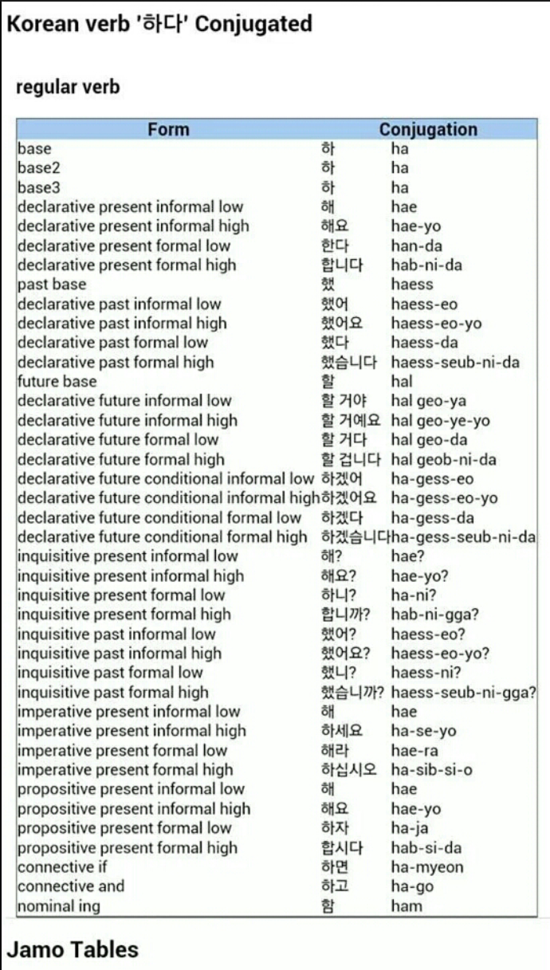
\includegraphics[height=\textheight]{verb_table}

\framebreak

One more issue; Zipf's Law. Top 10\% of vocabulary constitue of around 90\% of whole corpus. Most words are used only once or twice.

Therefore, defining vocabulary itself is not an easy task; just spliting with space does not make things work!

\framebreak

Now suppose we have a vocabulary(somehow). Is it done?

\begin{itemize}
\item world hello!
\item I like eat.
\end{itemize}

... Apparently not. There are more rules to be considered.

\framebreak

Through observation, we can conclude that

\begin{itemize}
\item Some words appear in similar position.
\begin{itemize}
\item I like (pizza|meat|flower|...)
\item I like (eat|run|...) : not
\end{itemize}
\item
\end{itemize}



\end{frame}

\begin{frame}{And Miles Make Path!}
\begin{itemize}
\item
\end{itemize}
\end{frame}




\begin{frame}[allowframebreaks]
\bibliographystyle{apalike}
\bibliography{reference}

\end{frame}

\end{document}